\documentclass[preprint]{aastex}

\usepackage{amsmath}
%\usepackage{graphicx}
%\usepackage{fullpage}
%\usepackage{multicol}
%\usepackage{natbib}
%\usepackage{amssymb}
%\usepackage{savesym}
%\usepackage{cancel}
%\usepackage{color}
%\usepackage{caption}
%\usepackage{subcaption}
%\usepackage{tabularx}
%\usepackage{mathtools}
%\usepackage{enumitem}
%\usepackage[font=small, labelfont=bf, labelsep=period, justification=justified]{caption}
%\usepackage{afterpage}
%\usepackage{hyperref}

%\usepackage{tikz}
%\def\checkmark{\tikz\fill[scale=0.4](0,.35) -- (.25,0) -- (1,.7) -- (.25,.15) -- cycle;}

%\bibliographystyle{unsrt}
%\setcitestyle{square}

%\providecommand{\e}[1]{\ensuremath{\times 10^{#1}}}
\newcommand{\e}[1]{\ensuremath{\times 10^{#1}}}

%\numberwithin{equation}{section}

\usepackage[T1]{fontenc}

\shorttitle{}
\shortauthors{Matthew Young}

\begin{document}

\title{A Cryogenic Testing Environment for SPT-3G}
\author{Matthew Young}
\affil{Astronomy \& Astrophysics Department, University of Toronto, ON}
\author{Supervised by: Keith Vanderlinde and Tyler Natoli}
%\affil{50 St. George Street\\Toronto, Ontario, Canada\\M5S 3H4}
%\email{young@astro.utoronto.ca}

\begin{abstract}
The next generation optical system for the South Pole Telescope, \textsc{spt-3g}, is set to be installed in early 2016.  This report outlines the fundamental science goals and operation behind \textsc{spt-3g}, and covers the continued development of a cryogenic testing environment at the Univeristy of Toronto for characterizing the next generation of detectors.  
\end{abstract}

%\keywords{key,words}


\section{Introduction}

The South Pole Telescope (\textsc{spt}), a 10 metre microwave telescope located at the geographic South Pole in Antarctica, is tasked with observing anisotropies in the Cosmic Microwave Background (CMB) \citep{spt_collaboration_south_2004}.  Optimized to operate in the band spanning from 75~GHz to 240~GHz, the telescope is capable of detecting the redshifted free streaming photons from the epoch of recombination.  The next generation optical system to be installed at the beginning of 2016, \textsc{spt-3g}, will contain over 16,000 polarization sensitive detectors, enabling high signal-to-noise mapping of both \textit{E}-mode and \textit{B}-mode CMB polarization anisotropies \citep{benson_spt-3g:_2014}.  In order to utilize this next generation of detectors to their full potential, a comprehensive suite of testing and characterizations must be performed throughout the \textsc{spt} collaboration.  Isolating the 2.7~K CMB spectrum and utilizing superconducting readout technologies, the detectors must operate at sub-Kelvin temperatures, requiring a cryogenic testing environment for wafer characterization to proceed at the University of Toronto.

\section{Background}

\subsection{\textsc{spt-3g}}
%This should be about the detectors and how they work, and how the cryostat is set up to test the detectors
%Maybe some science background as to why this project is interesting
Measurements produced by \textsc{spt-3g} will impact a range of cosmological fields, including inflationary theories, large-scale structure, and high-energy physics \citep{benson_spt-3g:_2014}.  The search for primordial \textit{B}-modes places constraints on the ratio of power in tensor perturbations to scalar perturbations, tied to the energy scale of inflation \citep{samtleben_cosmic_2007}.  Collected data will also be able to constrain the sum of neutrino masses, using information in the \textit{BB} lensed power spectrum to reduce the upper mass limit down to $\sim$0.06~eV, as well as addressing the neutrino mass hierarchy \citep{benson_spt-3g:_2014}.

Each \textsc{spt-3g} wafer fabricated by Argonne National Laboratory contains 217 pixels, with each pixel featuring a sinuous log-periodic antenna, microstrip inductor-capacitor (LC) filters, and six transition edge superconducting (TES) bolometers \citep{benson_spt-3g:_2014}.  A photograph of the pixel design is shown in Figure~\ref{pixel}.  The bolometers are responsible for detecting photons at band centres of either 95~GHz, 150~GHz, or 220~GHz for a given polarization, following the isolation of each signal by the LC filters.  As the TES bolometers are maintained in a superconducting phase transition through electro-thermal feedback \citep{benson_spt-3g:_2014}, a small increase in temperature due to the incident photons will result in a large change in resistivity.

Reading out the thermal loading of each bolometer individually introduces an unnecessary number of wires to the sub-Kelvin stage, and as such, \textsc{spt-3g} utilizes a frequency multiplexing readout system, enabling 64 bolometers to be addressed using a single wire \citep{dobbs_frequency_2012}.  By placing each resistive bolometer in series with a unique LC filter, an LCR resonator is formed \citep{henning_feedhorn-coupled_2012} that can be interrogated using its characteristic resonant frequency, allowing the warm electronics to perform readout in Fourier space.  A digital frequency multiplexing (DfMUX) \citep{dobbs_frequency_2012} system has been developed by McGill University, designed to deliver small amplitude excitations to each resonator with active digital feedback for nulling the subsequent signal.  The error in signal cancellation is then sensitively measured using superconducting quantum interference devices (SQUIDs) \citep{dobbs_frequency_2012}, inferring changes in the bolometer impedance and hence thermal loading.

\subsection{Experimental Setup}

The Long Wavelength Lab currently houses an Olympus 104 cryostat, designed and fabricated by \textit{High Precision Devices} (HPD) in Colorado.  Featuring a helium pulse tube refrigerator in conjunction with an adiabatic demagnetization refrigeration (ADR) system, the cryostat is capable of achieving temperatures as low as 35~mK.  These sub-Kelvin temperatures are realized through the ADR, consisting of two paramagnetic salt pills within a superconducting electromagnet, backed by the 3~K base temperature of the pulse tube.  By applying a large current to the electromagnet, magnetic domains within the salt pills will begin to align, freezing out a thermal degree of freedom within the salt pills.  Once fully magnetized, the current can be removed, allowing magnetic domains to realign themselves and reintroducing the thermal degree of freedom.  In accordance with the conservation of energy, the realignment process draws heat from the system, lowering the pills to sub-Kelvin temperatures.

The cryogenic testing environment also features an interactive control system and web interface, facilitating the measurement of system parameters such as temperature, pressure, and electromagnet current, as well as conducting the magnetization process.   An image of the current web interface is shown in Figure~\ref{web}.  Following demagnetization, a proportional-integral-derivative (PID) controller maintains the cold-stage temperature at a predetermined setpoint, capable of regulating temperatures of 100~mK for 100 hours.

\section{Research Plan}

As of September 2015, the HPD cryostat is fully operational, albeit with limited functionality and no facilities for conducting detector readout.  Before the testing and characterization of \mbox{\textsc{spt-3g}} detectors can begin, a number of modifications and additions must be made to the system.  First and foremost, an additional port must be opened on the cryostat, allowing for the installation of LC boards and SQUID cards along with an intermediate wire harness.  In conjunction, the readout chain for interfacing to an IceBoard running the DfMUX readout system must also be assembled, installed, and commissioned.  The readout hardware and code-base needs to be fully understood and established at a readily usable level to enable detector testing.

The project also entails improvements to the existing control system and web interface, allowing for a larger number of temperature sensors and greater control over the ADR magnetization process.  The previously developed code can also be integrated with the that of the DfMUX system, culminating in a singular system for operating both the cryostat and readout components.  As well as ultimately characterizing an \textsc{spt-3g} detector wafer, system parameters such as the cold stage thermal capacity, SQUID performance, and LC board behavior must also be determined.

%Addition of more temperature sensors and readout to web interface, and web interface having full control over magnetization process

%Finally the testing and characterization of detectors

\section{Current Progress \& Timeline}

To date, considerable progress has been made in preparing the cryostat for the installation of the DfMUX readout system.  Modified shield covers for the cryostat shell have been fabricated, with the pending delivery of flanges and an RF shielded box to accommodate the wire harness and LC cards.  In preparation for operating the readout system, a three-day training session was undertaken at McGill University, covering the hardware operation and corresponding python code-base, pyDfMUX.

Two additional Ruthenium Oxide temperature sensors have since been installed onto the ADR cold-stages, along with custom heaters to be used in characterizing the salt pill's thermal capacity.  Modifications have also been made to the web-interface, allowing for the readout of additional sensors to assist the magnetization process, and providing an interface for specifying the magnet's current, ramp rate, and soak time.  A timeline for the completion of the project is shown in Figure~\ref{gantt}.


%custom heaters

%training at Mcgill

%\acknowledgments
%I would like to acknowledge the acknowledgees.

%\bibliography{biball2}
\begin{thebibliography}{dummy}
\bibitem[Addison et al.(2015)]{addison_quantifying_2015}
Addison, G. E., Huang, Y., Watts, D. J., et al. 2015, {arXiv:1511.00055 [astro-ph]}

\bibitem[Samtleben et al.(2007)]{samtleben_cosmic_2007}
Samtleben, D., Staggs, S., Winstein, B. 2007, in Annual Review of Nuclear and Particle Science, 245-283

\bibitem[Bender et al.(2014)]{bender_digital_2014}
Bender, A. N., Cliche, J. F., Haan, T., et al. 2014, {arXiv:1407.3161 [astro-ph]}

\bibitem[Henning et al.(2012)]{henning_feedhorn-coupled_2012}
Henning, J. W., Ade, P., Aird, K. A., et al. 2012, {arXiv:1210.4969 [astro-ph]}

\bibitem[Dobbs et al.(2012)]{dobbs_frequency_2012}
Dobbs, M. A., Lueker, M., Aird., K. A., et al. 2012, Review of Scientific Instruments, 83, 7

\bibitem[Benson et al.(2014)]{benson_spt-3g:_2014}
Benson, B. A., Ade, P. A. R., Ahmed, Z., et al. 2014, {arXiv:1407.2973 [astro-ph]}

\bibitem[Ruhl et al.(2004)]{spt_collaboration_south_2004}
Ruhl, J. E., Ade, P. A. R., Carlstrom, J. E., et al. 2004, {arXiv:astro-ph/0411122}


	\begin{figure}
		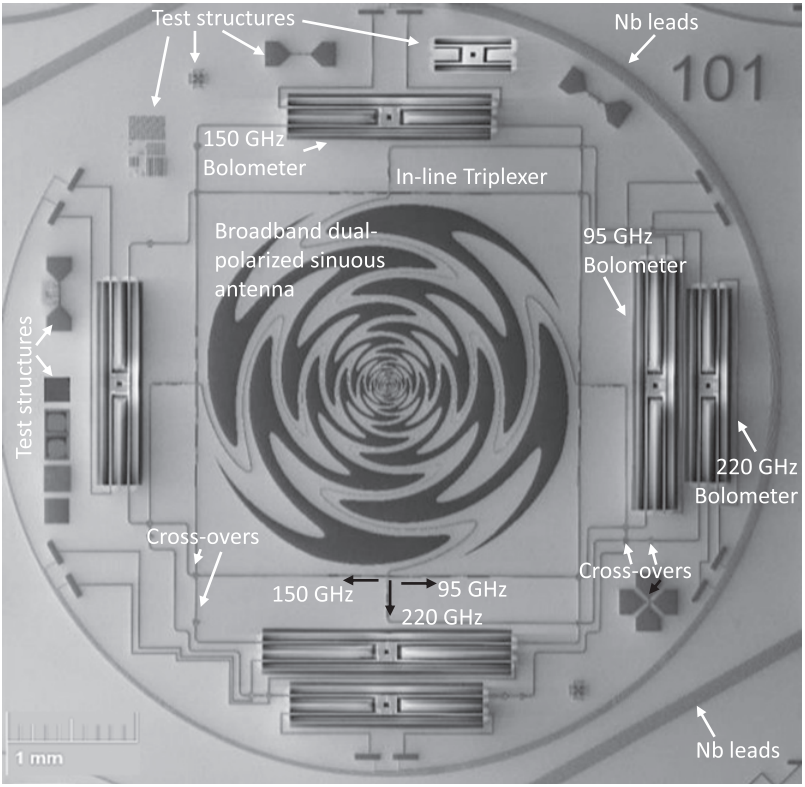
\includegraphics[width=\textwidth]{pixel}
		\centering
		\caption{Photograph of the tri-chroic (95/150/220 GHz) pixel featuring a sinuous log-periodic antenna. Also shown are the TES bolometers for each channel and polarization, along with the associated microstrip circuitry \citep{benson_spt-3g:_2014}.}
		\label{pixel}
	\end{figure}
	
	\begin{figure}
		\includegraphics[width=\textwidth]{cryo-server}
		\centering
		\caption{Screen shots of the cryostat web insterface, showing the overview panel (\textit{Left}) and control panel (\textit{Right}).  The overview panel displays the current system parameters, while the control panel is used to modify the magnetization cycle settings and begin the ADR process.}
		\label{web}
	\end{figure}

	\begin{figure}
		\includegraphics[height=20cm]{gantt2_vert}
		\centering
		\caption{Project timeline for the completion of a cryogenic testing environment, including testing of the DfMUX readout system and \textsc{spt-3g} wafer characterization.  The beginning and end of the  chart have been omitted for display purposes.}
		\label{gantt}
	\end{figure}

\end{thebibliography}

\end{document}


